\begin{figure*}[h]
\centering
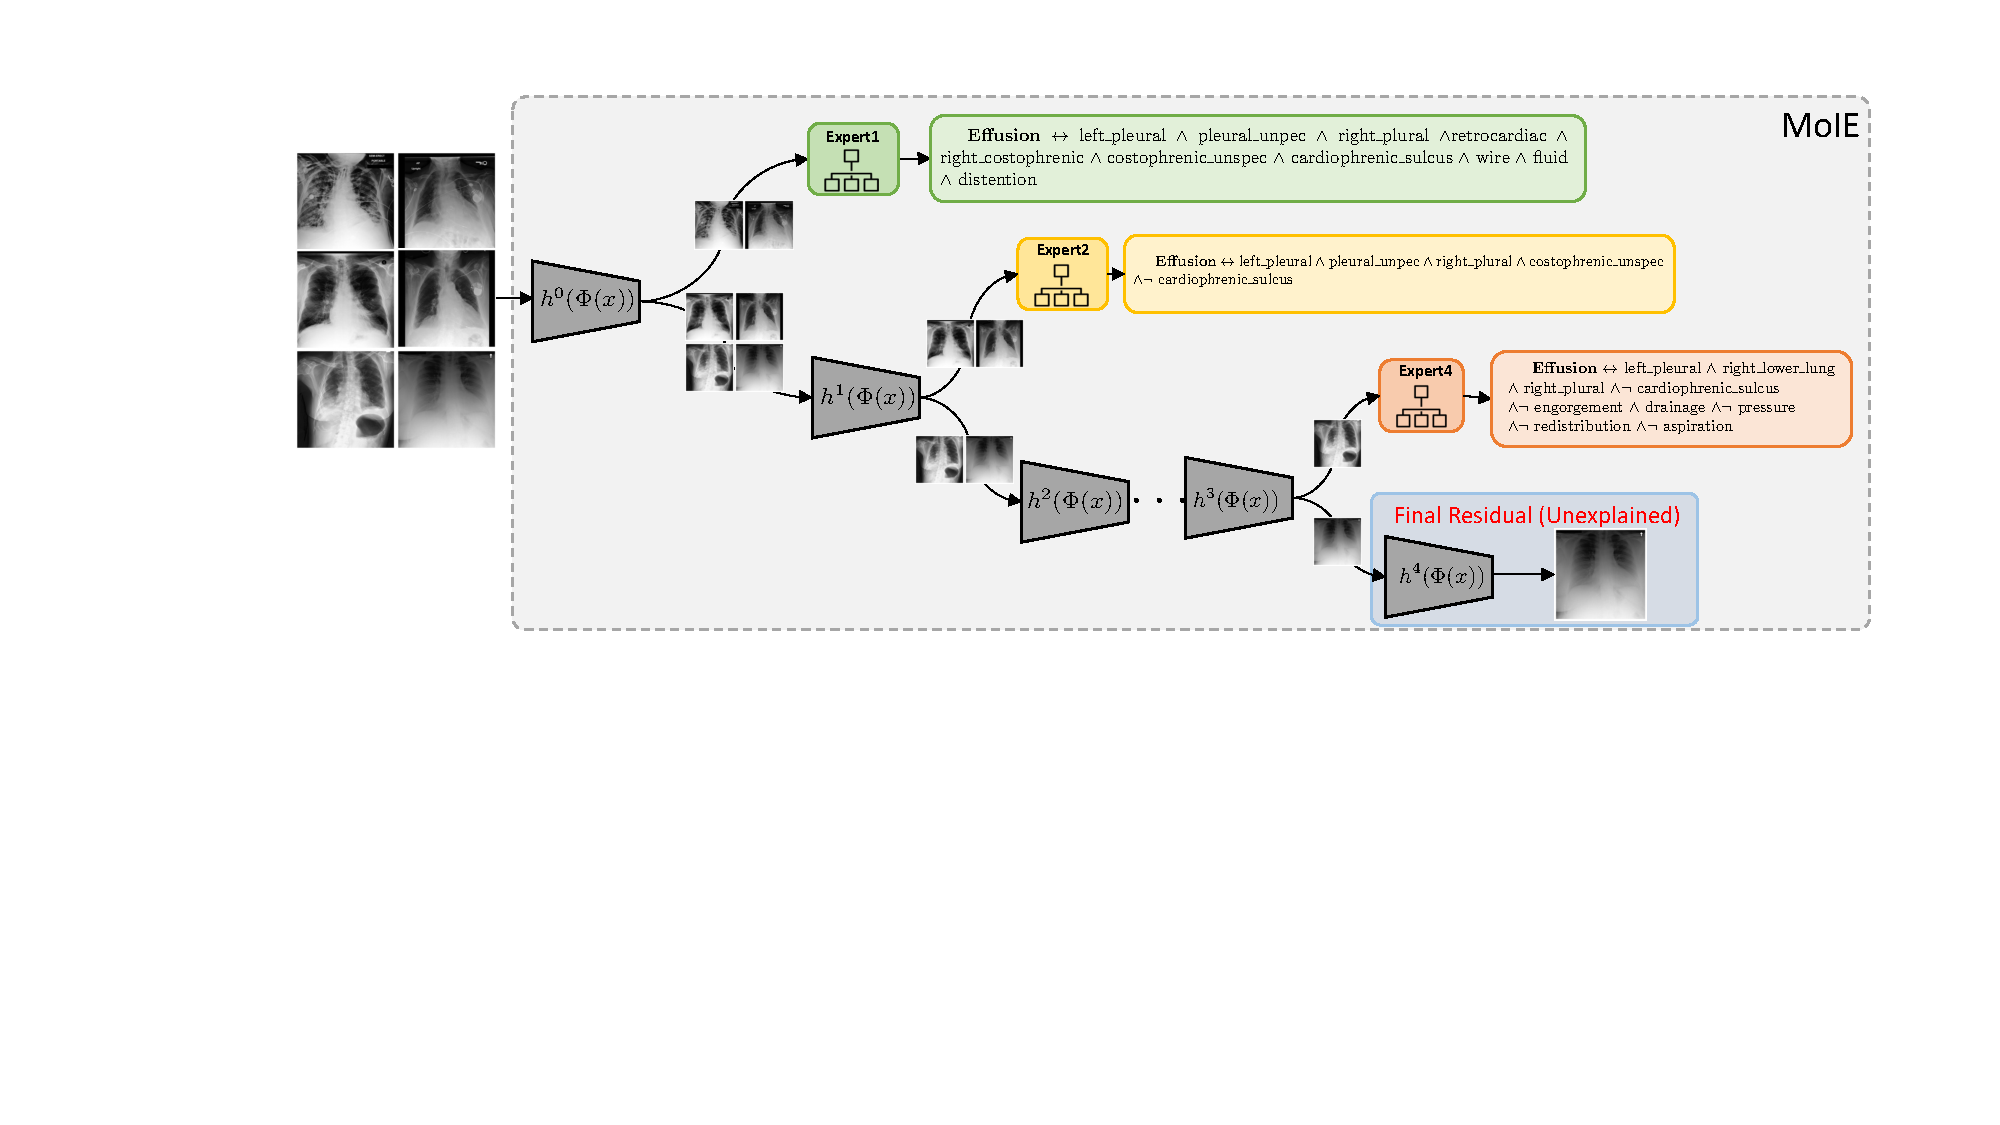
\includegraphics[width=1.0\textwidth]
{figures/Supp/mimic_concept_explanation.pdf}
\caption{Construction logical explanations of the samples of ``Effusion'' in the MIMIC-CXR dataset for various experts in MoIE at inference. The final residual covers the unexplained sample, which is ``harder'' to explain (indicated in \emph{red}).}
\label{fig:mimic_concept_explanation}
\end{figure*}

\begin{figure*}[h]
\centering
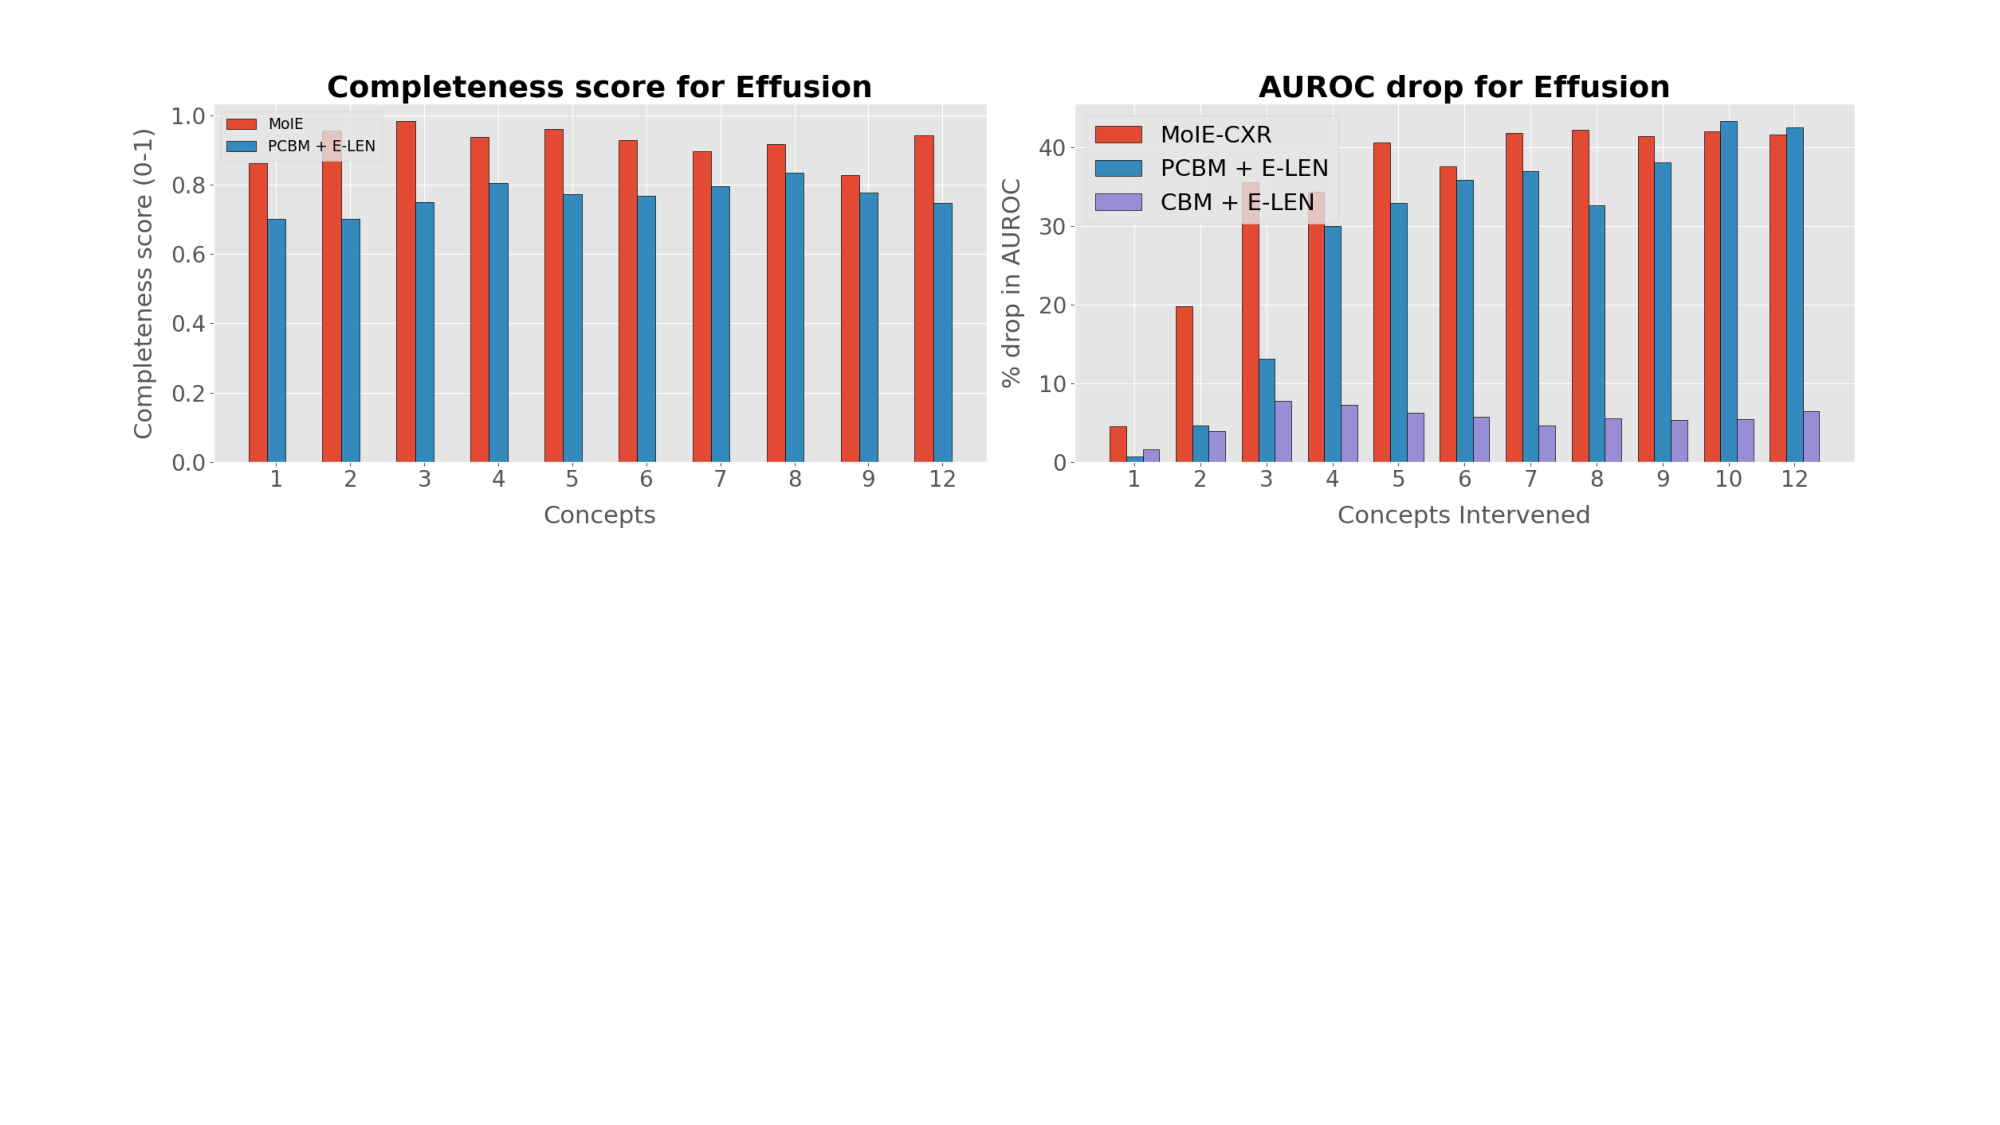
\includegraphics[width=1.0\textwidth]
{figures/Supp/mimic_concept_quant.pdf}
\caption{\textbf{(a)} Completeness scores for different significant concepts of Effusion.  \textbf{(b)} Drop in AUROC by zeroing out the concepts for Effusion.}
\label{fig:mimic_concept_quant}
\end{figure*}

\begin{figure*}[h]
\centering
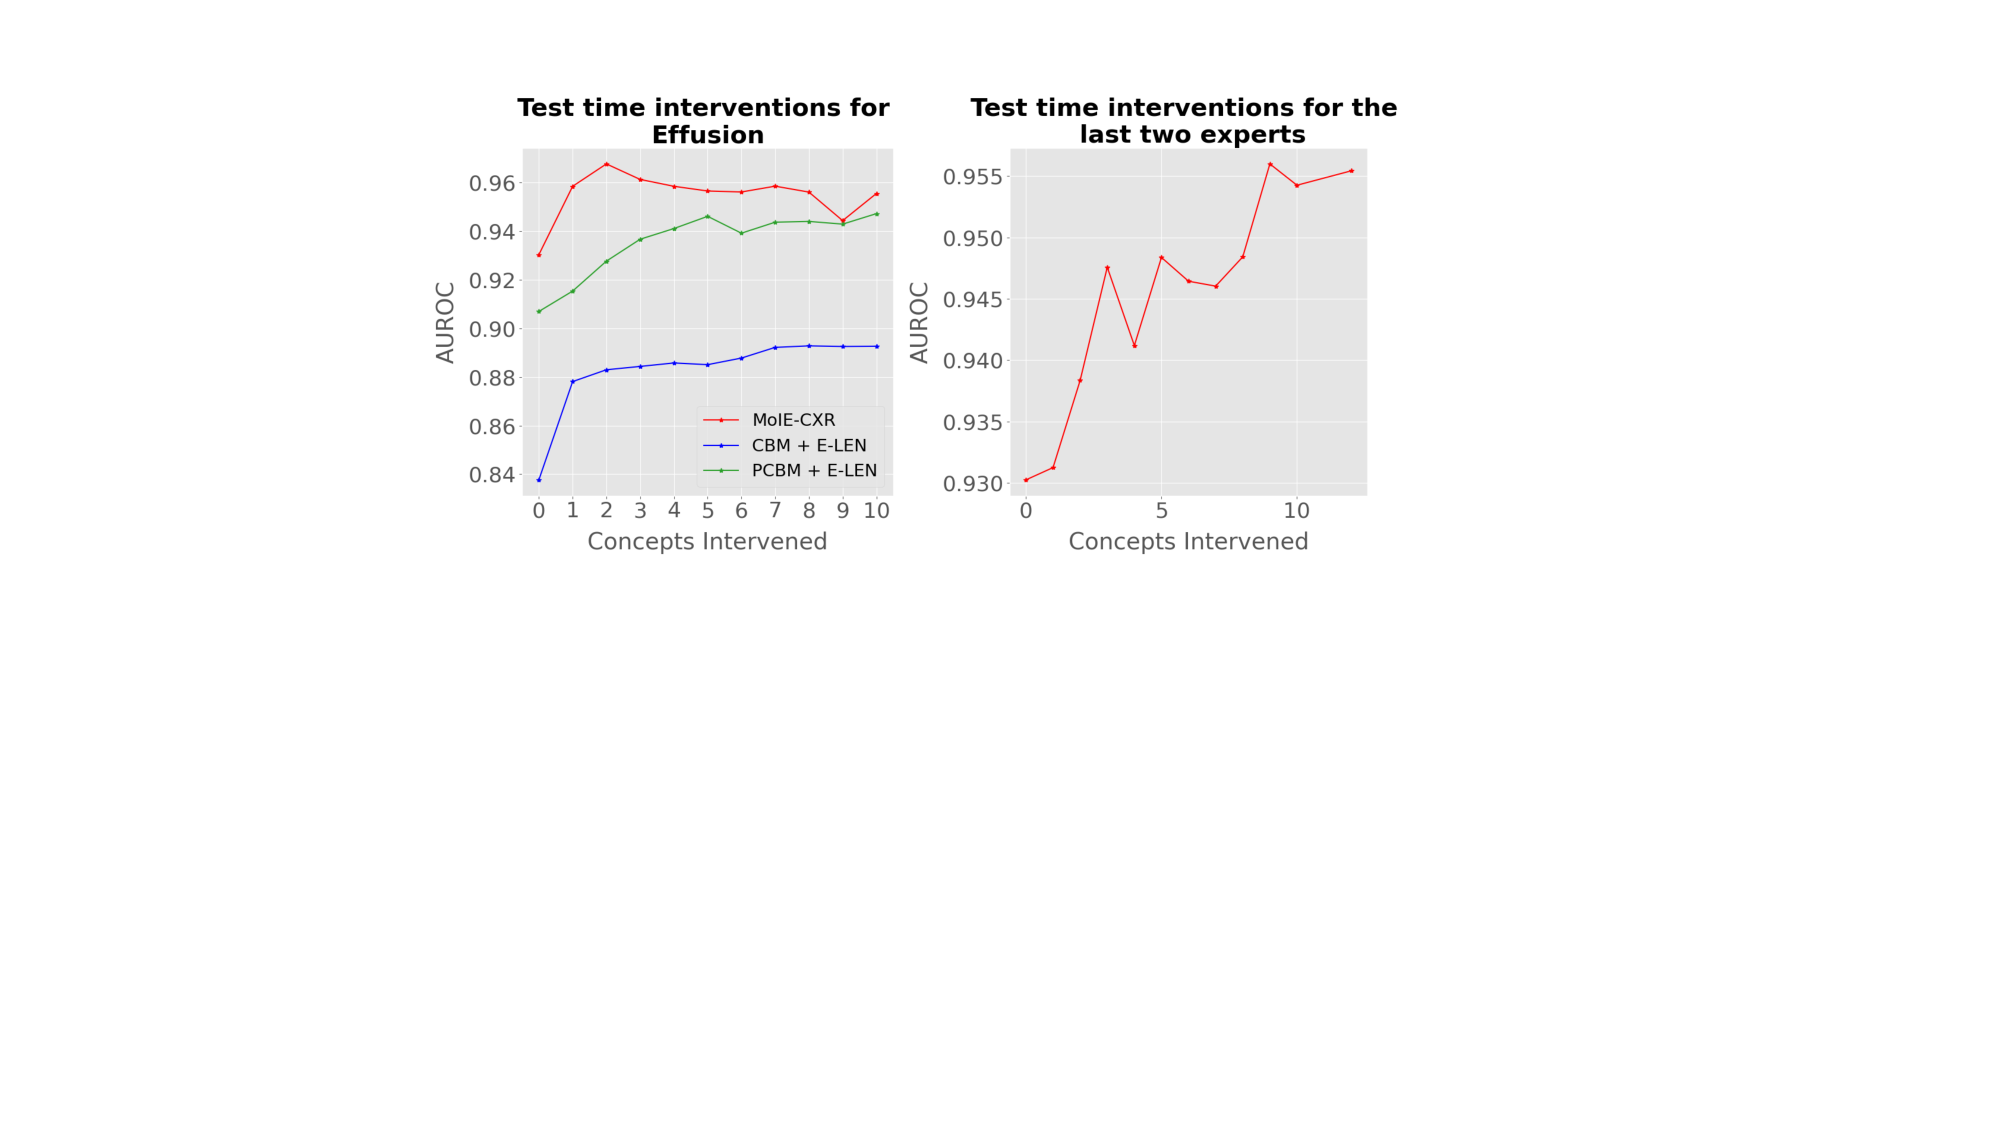
\includegraphics[width=1.0\textwidth]
{figures/Supp/mimic_concept_tti.pdf}
\caption{\textbf{(a)} Test time interventions of different concepts on all samples for Effusion.
\textbf{(b)} Test time interventions of different concepts on only the ``hard'' samples covered by the last two experts for Effusion}
\label{fig:mimic_concept_tti}
\end{figure*}

~\cref{fig:mimic_concept_explanation} demonstrates the diversity of instance-specific local FOL explanations of different concepts of MoIE and the final residual.~\cref{fig:mimic_concept_quant}(a) shows the completeness scores for different concepts.~\cref{fig:mimic_concept_quant}(b) shows the drop in AUROC while zeroing out different concepts. ~\cref{fig:mimic_concept_tti}(a) shows test time interventions of different concepts on all samples. ~\cref{fig:mimic_concept_tti}(b) shows test time interventions of different concepts on only the ``hard'' samples covered by the last two experts.


